\documentclass[border=4pt]{standalone}
\usepackage{tikz}
\usetikzlibrary{positioning, arrows.meta, shapes.geometric}
\usepackage{xcolor}

\definecolor{accent}{HTML}{4A90D9}
\definecolor{navy}{HTML}{1E2761}
\definecolor{leafgreen}{HTML}{27AE60}
\definecolor{purple}{HTML}{8E44AD}
\definecolor{grayDark}{HTML}{4A5568}

\begin{document}
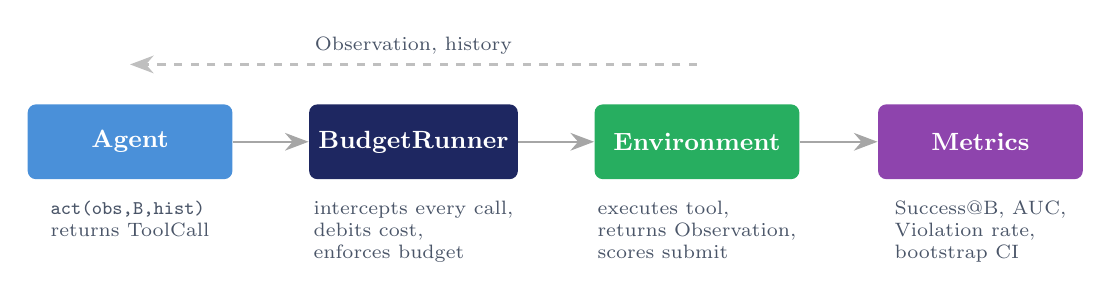
\begin{tikzpicture}[
    box/.style={rectangle, rounded corners=3pt, minimum height=0.95cm, minimum width=2.6cm,
                font=\small\bfseries, text=white, draw=none, align=center},
    arr/.style={-{Stealth[length=3mm]}, thick, gray!70},
    label/.style={font=\scriptsize, text=grayDark, align=left}
  ]
  \node[box, fill=accent]    (agent)   at (0,0)    {Agent};
  \node[box, fill=navy]      (runner)  at (3.6,0)  {BudgetRunner};
  \node[box, fill=leafgreen] (env)     at (7.2,0)  {Environment};
  \node[box, fill=purple]    (metrics) at (10.8,0) {Metrics};

  \draw[arr] (agent)  -- (runner);
  \draw[arr] (runner) -- (env);
  \draw[arr] (env)    -- (metrics);

  \node[label, below=4pt of agent.south]   {\texttt{act(obs,B,hist)}\\returns ToolCall};
  \node[label, below=4pt of runner.south]  {intercepts every call,\\debits cost,\\enforces budget};
  \node[label, below=4pt of env.south]     {executes tool,\\returns Observation,\\scores submit};
  \node[label, below=4pt of metrics.south] {Success@B, AUC,\\Violation rate,\\bootstrap CI};

  \draw[arr, dashed, gray!50] (env.north) ++(0,0.5) -- ++(-7.2,0)
        node[midway, above, label] {Observation, history};
\end{tikzpicture}
\end{document}
